\documentclass[12pt]{article}

\usepackage{amsmath}
\usepackage[margin=0.75in]{geometry}
\usepackage[numbers]{natbib}
\usepackage{physics}
\usepackage[hyphens]{url}
\usepackage[labelformat=simple,position=b]{subcaption}
\renewcommand\thesubfigure{(\alph{subfigure})}
\usepackage{fancyhdr}
\pagestyle{fancy}
\fancyhf{}
\rhead{Team 10}
\lhead{Week 1: Trapped ions}
\rfoot{Page \thepage}

\usepackage{graphicx}
\graphicspath{
	{figures}
}

\usepackage[hidelinks]{hyperref}


\renewcommand{\phi}{\varphi}


\title{Week 1: Simulating quantum advantage with trapped ions}
\author{Team 10: Alexander (Sandy) Bell, Na Young Kim, Sushanta Mitra, Ushnish Ray, Ming-Tso Wei}
\date{\today}


\begin{document}

\maketitle

%\thispagestyle{empty}


\section*{Introduction}

We put all the functions for the coding tasks in the script \texttt{assignment.jl}.

%% Ray: do you need to explain some of your code about the modification of "run" function, like the use of MersenneTwister.


\section*{Task 1}

In this task, we create a function \texttt{getAmp2} to calculate the probability $P(x)= \abs{\ip{x}{\psi}}^2$ of each bit-string $x$ showing as a dot in the speckle pattern by taking the dot product between the bit-string and $\ket{\psi}$ from the \texttt{run} function given in the script \texttt{run\_random\_circuit.jl}. In Fig. \ref{fig:speckle}, we plot 16 different combinations of $N$ and circuit depths, where $N$ varies from 2 to 5, and the depths include 4, 16, 32, and 64. These patterns are plotted by the function \texttt{speckles()}. One can find that some bitstrings are much more likely to occur than others, especially when $N$ is larger. The location $x$ with highest probability seems to distribute randomly.

\begin{figure}
	\centering
	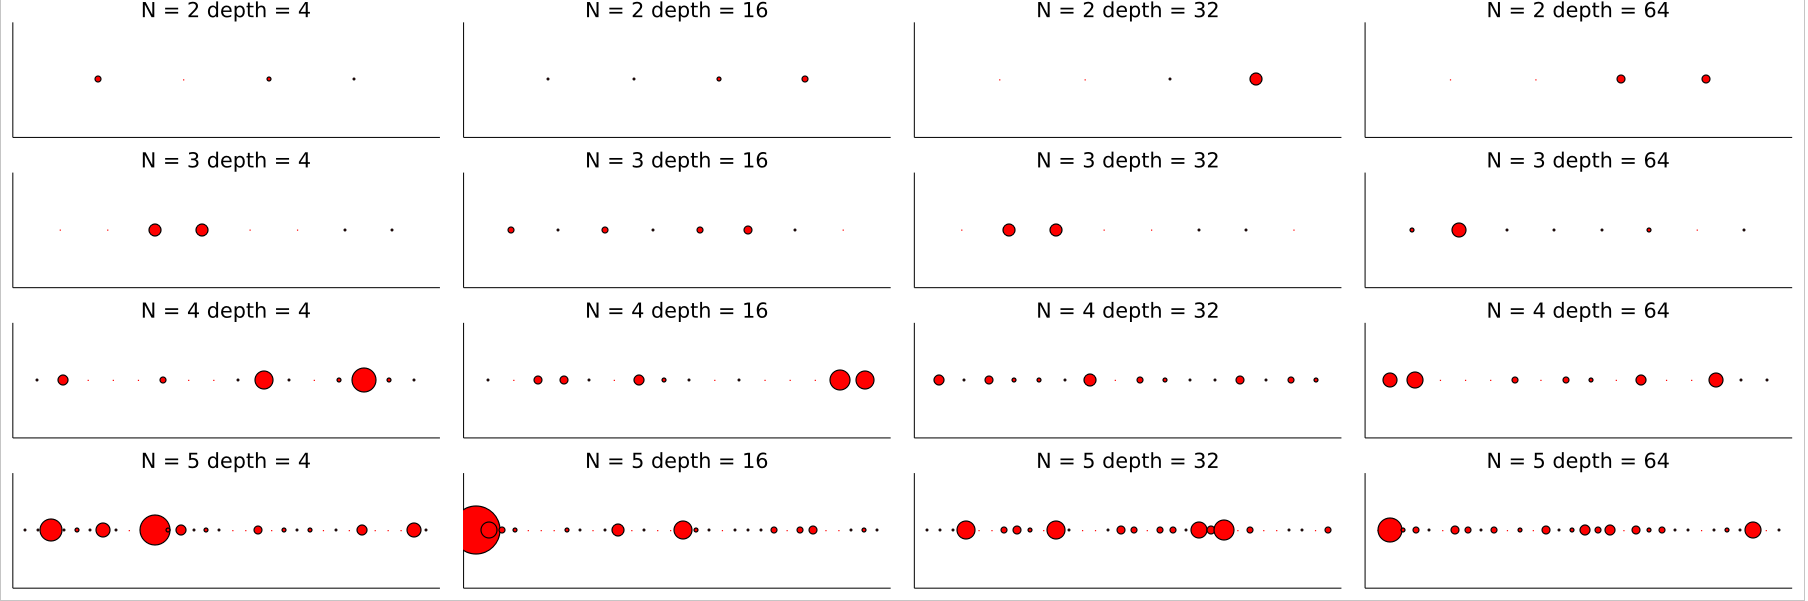
\includegraphics [width=\linewidth] {figures/Task_1a}
	\caption{
		``Speckle patterns'' displaying the probabilities of obtaining with $N=2$ to 5 and depths of 4, 16, 32, and 64.
	}
	\label{fig:speckle}
\end{figure}

We also make a function \texttt{studyBondDim} to calculate the bond dimension in the bonus problem by using the built-in function \texttt{maxlinkdim} in ITensor. In Fig. \ref{fig:bonddim}, we plot  the bond dimensions as a function of circuit depth at several values of $N$. The bond dimension saturates at a higher circuit depth when $N$ is larger. % I'm not sure what it means here actually.

\begin{figure}
	\centering
	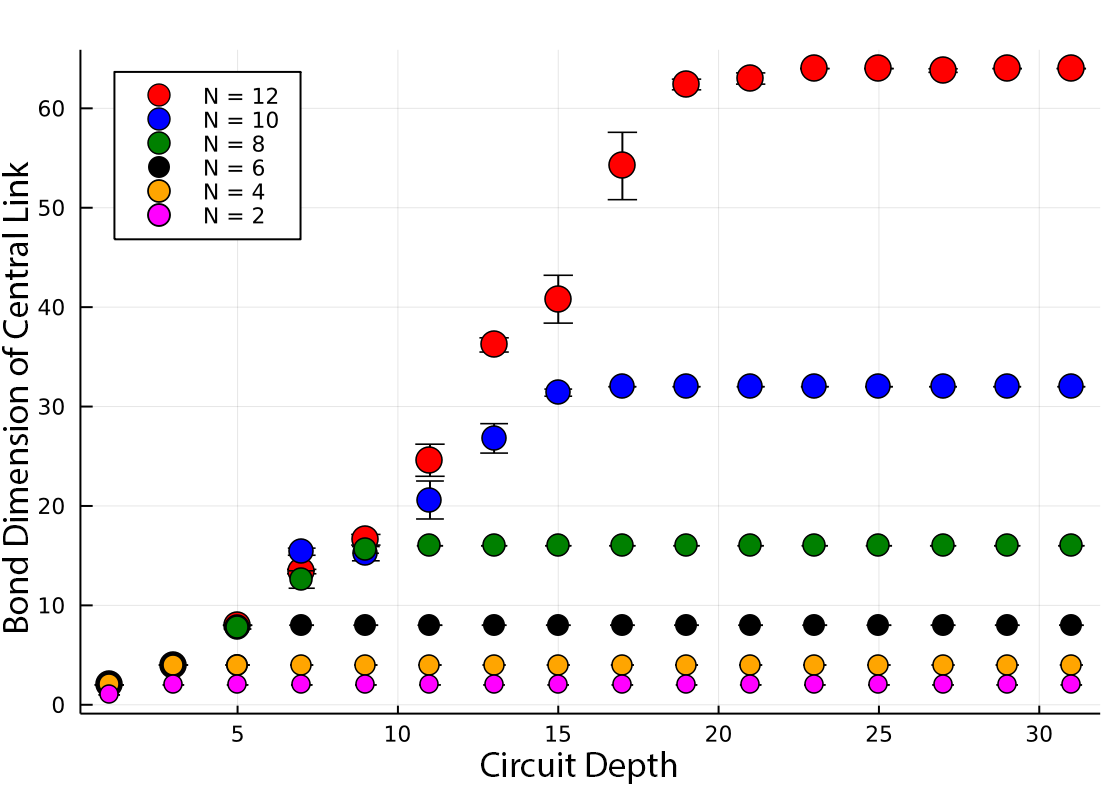
\includegraphics [width=0.8\linewidth] {figures/Task1b}
	\caption{
		The bond dimensions of central links as a function of circuit depth at different numbers of qubits. At a 
	}
	\label{fig:bonddim}
\end{figure}

%% Need some discussion for the connection to entanglement entropy here.


\section*{Task 2}

To consider a single random bit flip, we modified the given \texttt{run} function by adding an argument \texttt{wbitflip}. If \texttt{wbitflip} is \texttt{True}, we assign a bit flip at a random location \texttt{bitloc} in the modified \texttt{run} function. In the \texttt{bitFlipCompile} function, we let \texttt{wbitflip=True} and plot 16 different speckle patterns generated from a single bit flip error of a single gate and collect them into a collage, as shown in Fig. \ref{fig:bitflip}.

\begin{figure}
	\centering
	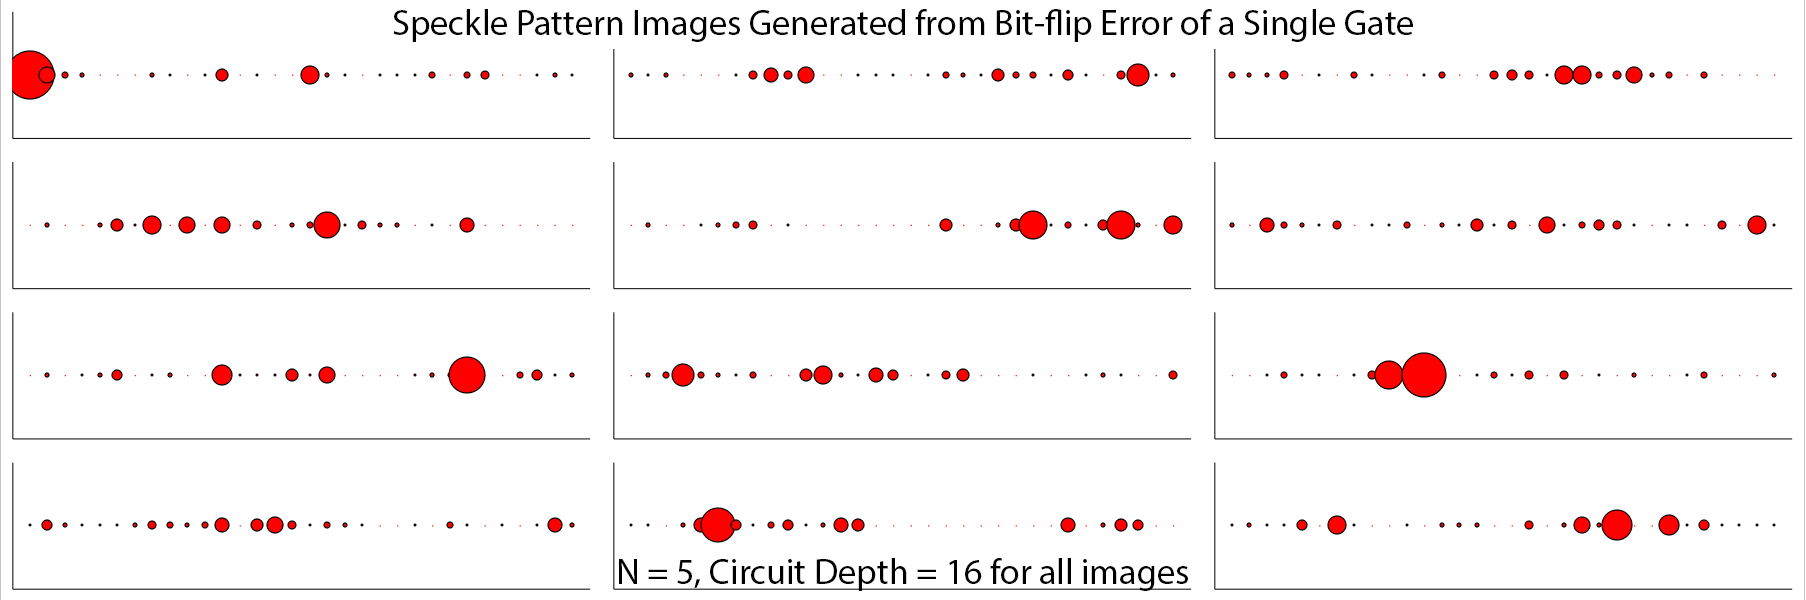
\includegraphics [width=\linewidth] {figures/Task2}
	\caption{
		 ``Speckle patterns'' displaying the probabilities of obtaining each of the 16 possible outcomes when sampling a 5-qubit circuit with a bit flip error occurred at a random location.
	}
	\label{fig:bitflip}
\end{figure}

\section*{Task 3}

In this task, we create a function \texttt{cgfScalingSingle} to calculate the cumulative distribution function (CDF) by numerically summing or integrating the probability distribution. Then we use the function \texttt{cgfScaling} to plot the CDF values with different depths and compare them with the theoretical value $1-e^{-2^Np}$, as shown in Fig. \ref{fig:cdf}

\begin{figure}
	\centering
	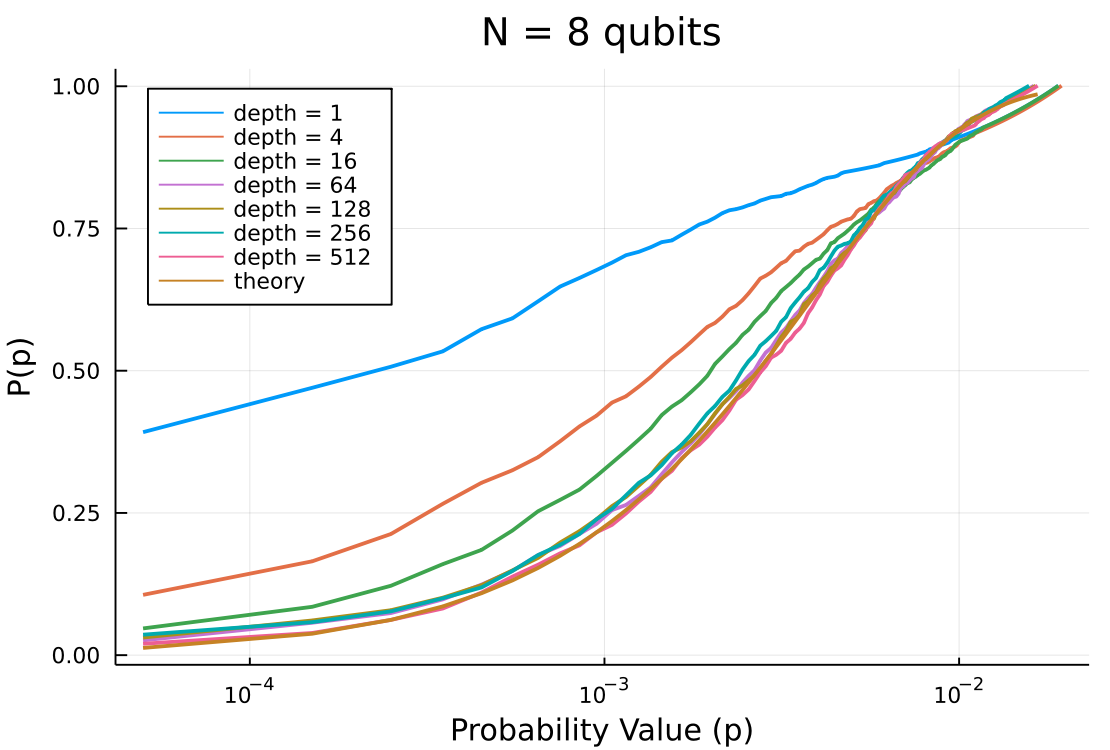
\includegraphics [width=0.8\linewidth] {figures/Task3}
	\caption{
		Calculated CDF as a function of the probability values $p$ in log scale at different circuit depths in an 8-qubit circuit. When the depth is larger, the CDF converges toward the theoretical value $1- e^{-2^Np}$.
	}
	\label{fig:cdf}
\end{figure}

\section*{Task 4}

In the function \texttt{crossEntropyValue}, we calculate the linear cross-entropy benchmarking (XEB) fidelity $\mathcal{F}_\mathrm{XEB}$, defined in Eq. (1) of the instruction. In Fig. \ref{fig:task4}, the function \texttt{crossEntropy} assembles the results at different $\Delta \Theta$ and plots the $\mathcal{F}_\mathrm{XEB}$ as a function of $\Delta \Theta$.

In the function \texttt{crossEntropywDavg}, $\mathcal{F}_\mathrm{XEB}$ is calculated by averaging over a certain number of samples $s$. In Figs. \ref{fig:XEBfidelity} (b) - (d), we calculate the XEB fidelity $\mathcal{F}_\mathrm{XEB}$ when performing the averages over a number of samples $s$. A peak occurs near $\Delta \Theta=\pi$.


\begin{figure}
	\centering
	\begin{subfigure}[t]{0.42\textwidth}
		\centering
		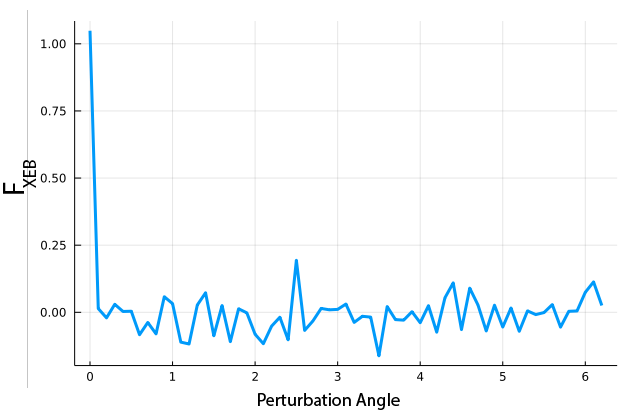
\includegraphics[width=\linewidth]
		{figures/Task4}
		\subcaption{\label{fig:task4}}
	\end{subfigure}%a
	\begin{subfigure}[t]{0.42\textwidth}
		\centering
		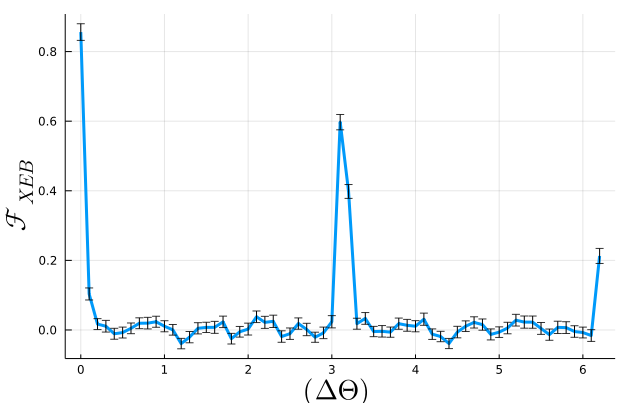
\includegraphics[width=\linewidth]
		{figures/Task4b_N_4_d_128_s_200_fg}
		\subcaption{\label{fig:task4b_N4}}
	\end{subfigure}%b
	
	\begin{subfigure}[t]{0.42\textwidth}
		\centering
		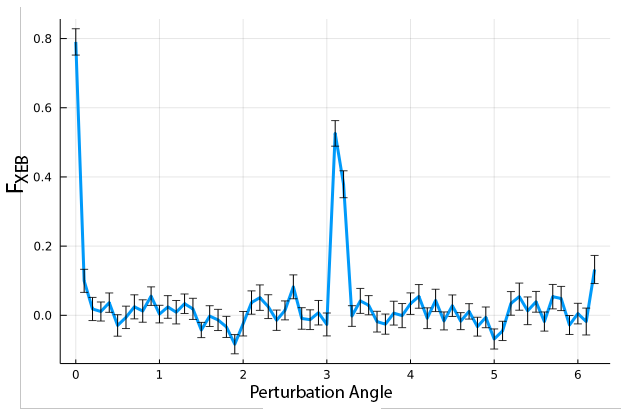
\includegraphics[width=\linewidth]
		{figures/task4b_N_8_d_128_s_50_fg}
		\subcaption{\label{fig:task4b_N8}}
	\end{subfigure}%c
	\begin{subfigure}[t]{0.42\textwidth}
		\centering
		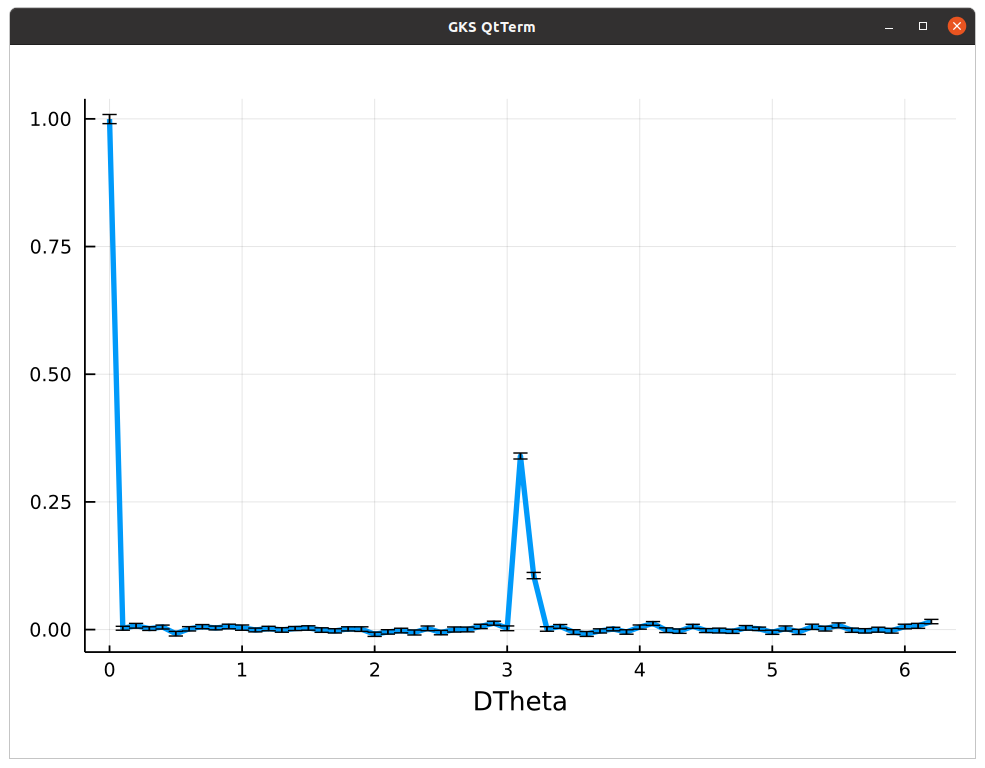
\includegraphics[width=\linewidth]
		{figures/Task4b_N_10_d_128_s_50_fg}
		\subcaption{\label{fig:task4b_N10}}
	\end{subfigure}%d
	\caption{
		The crossed entropy benchmarking fidelity $\mathcal{F}_\mathrm{XEB}$ calculated as a function of the perturbation angle $\Delta \Theta$ in a unit of radians at different numbers of qubit $N$, circuit depths $d$, and numbers of samples $s$. \subref{fig:task4} $N$=8, $d$=512, without averaging; \subref{fig:task4b_N4} $N$=4, $d$= 128, $s$=200; \subref{fig:task4b_N8} $N$=8, $d$=128, $s$=50; \subref{fig:task4b_N10} $N$=10, $d$=128, $s$=50.
	}
	\label{fig:XEBfidelity}
\end{figure}

\section*{Business Application}


\end{document}
